\newpage
\section{Arquitectura híbrida para la generación de Django ORM}
\label{sec:segundo-prototipo}

A partir de los hallazgos y limitaciones identificadas en el primer prototipo —donde la inferencia puramente neuronal de CodeT5 mostró inestabilidad y falta de determinismo al traducir relaciones complejas y Claves Primarias (PK)—, se diseñó e implementó un segundo prototipo basado en una \textbf{arquitectura híbrida}.

\subsection{Arquitectura general y justificación de diseño}
\label{subsec:p2-arquitectura}

La arquitectura híbrida establece una clara separación de responsabilidades entre el modelo generativo y una capa de procesamiento determinístico en Python:
\begin{itemize}
    \item \textbf{CodeT5 (Especializado en Atributos):} Mantiene la responsabilidad de traducir únicamente el conjunto de atributos simples de una sola entidad a sus correspondientes campos de Django ORM (ej., \texttt{IntegerField}, \texttt{CharField}).
    \item \textbf{Capa Determinística (Especializada en Estructura y Relaciones):} Procesa de forma algorítmica la validación del contrato, el cálculo de PK simples y compuestas, la propagación de llaves, la aplicación de reglas relacionales para los \textit{Idioms}, el manejo de restricciones de integridad y la construcción final del archivo \texttt{models.py}.
\end{itemize}

Ambos componentes interactúan exclusivamente mediante el intercambio de estructuras de datos (arreglos de campos en JSON) sin compartir espacio de memoria o código, garantizando un acoplamiento débil.

\begin{figure}[htbp]
    \centering
    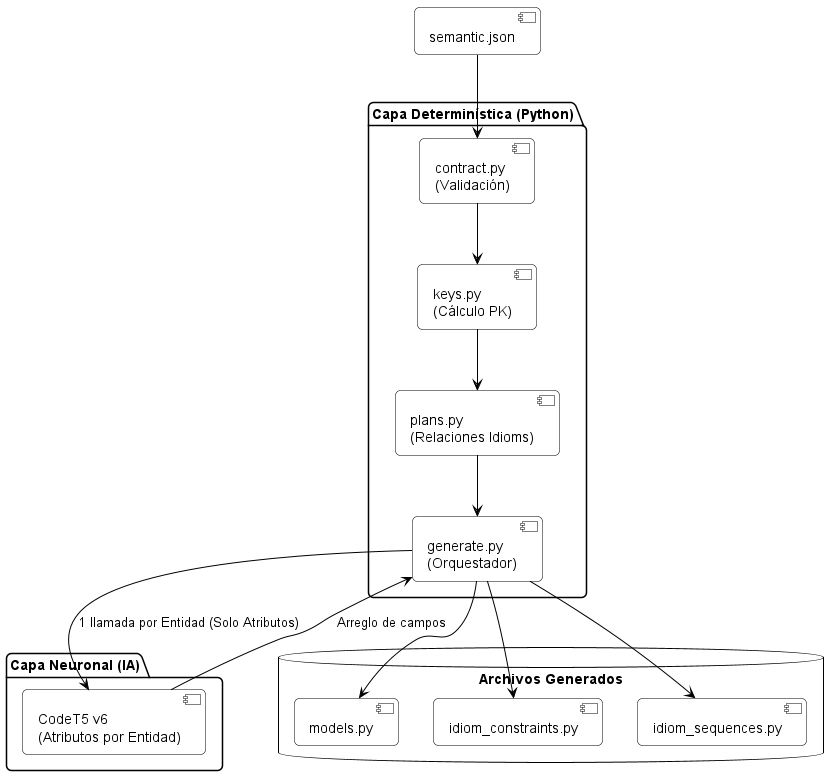
\includegraphics[width=0.65\textwidth]{diagramas/arquitectura_hibrida_p2/arquitectura_hibrida_p2.png}
    \caption{Arquitectura híbrida combinando CodeT5 y la capa determinística en Python.}
    \label{fig:arquitectura-hibrida-p2}
\end{figure}

\subsection{Evolución del modelo de IA y Dataset v6}
\label{subsec:p2-dataset-v6}

Para optimizar el rendimiento de CodeT5, se modificó el alcance del modelo. Mientras que en la versión V4 se intentó traducir el JSON completo del diagrama (obteniendo degradación progresiva al aumentar las relaciones), en la \textbf{Versión V6} el contrato del modelo se simplificó para procesar **una sola entidad por llamada**.

\subsubsection{Construcción del Dataset v6}
Se desarrolló un generador sintético automatizado en Python (\texttt{dataset\_generator.py}, véase Anexo~\ref{anx:dataset-v6}) que estructuró los datos bajo los siguientes criterios:

\begin{itemize}
    \item \textbf{Instrucción Fija:} \textit{``Generate Django model fields from the entity attributes.''}
    \item \textbf{Formato de Entrada Compacto:} Eliminación de metadatos no esenciales (identificadores y relaciones), enviando únicamente el nombre de la entidad y sus atributos (ej., \texttt{\{"name":"User", "attributes":[\{"name":"age", "type":"int"\}]\}}).
    \item \textbf{Mapeo Semántico Desacoplado:} Se asignaron tipos de datos semánticos al azar independientes del nombre del atributo para que la red neuronal aprendiera la relación tipo-campo y no una memorización por nombre.
    \item \textbf{División sin Solapamiento:} Se dividieron 300 ejemplos con semilla fija en conjuntos de Entrenamiento (200), Validación (50) y Fuera de Distribución / OOD (50) con nombres que jamás aparecieron en el entrenamiento.
\end{itemize}

\subsubsection{Entrenamiento y Resultados de Inferencia (v6)}
El entrenamiento se ejecutó en Google Colab con aceleración GPU (NVIDIA T4). Evaluado con 50 ejemplos en validación y 50 en pruebas OOD, el modelo alcanzó un **$100\%$ de Exact Match**, logrando copiar correctamente nombres, clases de campo y la cantidad exacta de atributos.

Un experimento negativo de control confirmó la hipótesis de diseño: al intentar enviar múltiples entidades o el JSON completo dentro del mismo \textit{prompt}, el modelo perdió atributos y confundió nombres de clases con campos. Por ello, se consolidó la regla de **una llamada por entidad**.

\subsection{Capa determinística de traducción}
\label{subsec:p2-capa-deterministica}

Desarrollada en Python puro sin dependencias de librerías de \textit{Deep Learning}, la capa determinística (\texttt{deterministic\_layer/}) se validó mediante 63 pruebas unitarias y consta de los siguientes componentes secuenciales:

\begin{enumerate}
    \item \textbf{\texttt{contract.py} (Validación):} Analiza la sintaxis del \texttt{semantic.json}, validando palabras reservadas, ausencia de caracteres especiales no ASCII, consistencia en roles y detección de dependencias circulares.
    \item \textbf{\texttt{keys.py} (Cálculo de PK y Propagación):} Realiza el ordenamiento topológico del modelo conceptual. Asigna \texttt{AutoField} a entidades sin identificador explícito, o define la PK manual según los atributos especificados. Maneja las relaciones identificantes (donde la PK del padre se propaga a la PK del hijo).
    \item \textbf{\texttt{plans.py} (Traducción de Relaciones):} Aplica las reglas estructurales para los 6 patrones de \textit{Idioms}:
    \begin{itemize}
        \item \textit{Classification:} Genera un campo \texttt{ForeignKey} en la entidad origen con regla \texttt{SET\_NULL}.
        \item \textit{Master-Detail / Composition:} Propaga la clave foránea con borrado en cascada (\texttt{CASCADE}) integrada dentro de la clave primaria compuesta del hijo.
        \item \textit{Is-A:} Genera un \texttt{OneToOneField(primary\_key=True)} en el subtipo apuntando al supertipo.
        \item \textit{Historic-Reflexive:} Genera dos claves foráneas con \texttt{CASCADE} hacia la entidad reflexiva correspondientes a cada rol definido.
    \end{itemize}
    \item \textbf{\texttt{generate.py} (Orquestador):} Valida el diagrama de entrada, invoca a CodeT5 para la generación de atributos, verifica los arreglos resultantes con \texttt{fields\_check.py} y ensambla el archivo \texttt{models.py} final.
\end{enumerate}

\subsection{Soluciones a las limitaciones del ORM de Django y PostgreSQL}
\label{subsec:p2-limitaciones-django}

Durante la implementación se identificaron dos restricciones críticas del ORM de Django frente a modelos conceptuales complejos:
\begin{enumerate}
    \item Django no soporta de forma nativa Claves Foráneas que apunten a modelos con Claves Primarias Compuestas.
    \item El uso de \texttt{ForeignObject} provee navegación a nivel de software pero no genera la restricción de integridad en la base de datos relacional.
\end{enumerate}

Para resolver estos desafíos, se desarrollaron e integraron los siguientes componentes técnicos de soporte:

\subsubsection{Restricción de Claves Foráneas Compuestas (\texttt{CompositeForeignKeyConstraint})}
Se implementó la clase \texttt{CompositeForeignKeyConstraint} (Anexo~\ref{anx:idiom-constraints}) heredada de \texttt{BaseConstraint}. Esta subclase se declara dentro del bloque \texttt{Meta.constraints} del modelo Django. Al ejecutar \texttt{makemigrations} y \texttt{migrate}, genera directamente la instrucción SQL equivalente:
\begin{verbatim}
FOREIGN KEY (a, b) REFERENCES tabla_padre (a, b) DEFERRABLE INITIALLY DEFERRED
\end{verbatim}

\subsubsection{Generación de Secuencias para PK Compuestas (\texttt{SequentialIdMixin})}
Dado que un campo \texttt{AutoField} no puede formar parte de una \texttt{CompositePrimaryKey} en Django, se desarrolló el mixin \texttt{SequentialIdMixin} (Anexo~\ref{anx:idiom-sequences}). Este componente intercepta el método \texttt{save()} del modelo, aplica un bloqueo de tabla concurrente (\texttt{LOCK TABLE ... IN EXCLUSIVE MODE}) y asigna de manera segura el identificador consecutivo dentro de la transacción, garantizando el cumplimiento del principio ACID bajo concurrencia.

\subsection{Verificación y pruebas del sistema}
\label{subsec:p2-verificacion}

El funcionamiento integral del segundo prototipo se verificó mediante tres escenarios de prueba:

\begin{itemize}
    \item \textbf{Verificación en PostgreSQL (8 Tablas):} Se procesó un modelo complejo (\texttt{semantic2.json}) que abarcaba la totalidad de los 6 \textit{Idioms}. Tras ejecutar la migración, la inspección del ERD en pgAdmin confirmó la correcta generación de las claves primarias compuestas y las restricciones relacionales.
    \item \textbf{Prueba de Concurrencia (App \texttt{seqtest}):} Se ejecutó un test de estrés con 8 hilos concurrentes realizando 10 inserciones cada uno (80 registros en total). Se comprobó la generación estricta de IDs contiguos e incrementales sin colisiones ni interbloqueos.
    \item \textbf{Suites de Pruebas Unitarias:} 63 pruebas unitarias de la capa determinística superadas al $100\%$.
\end{itemize}